%!TeX root=../tese.tex
%("dica" para o editor de texto: este arquivo é parte de um documento maior)
% para saber mais: https://tex.stackexchange.com/q/78101/183146

%% ------------------------------------------------------------------------- %%
\chapter{Decisões de \textit{Design}}
\label{cap:processo de desenvolvimento}
\section{Ideias Iniciais}

Inicialmente, foram avaliadas diversas possibilidades de gêneros para o jogo. O Artigo de~\citet{DynamicDiffAdjustment} mostra as vantagens de uma abordagem baseada em colocar o jogador em uma situação onde enfrenta diversos inimigos, em oposição a um jogo de luta, onde ele poderia enfrentar apenas um, ou jogos de quebra-cabeça, onde normalmente não existem inimigos. Para isso, foi desenvolvido um pequeno protótipo no estilo \textit{top-down}\footnote{
    Jogos definidos pelo ângulo de visão do jogo, vendo o personagem por cima, em oposição à visão pelos lados, usada em jogos como \textit{Super Mario Bros}.
}, onde o personagem principal podia atirar em qualquer direção usando uma gama de armas selecináveis, em uma \textit{arena}. Isso é, ele se encontrava em uma fase fechada, com apenas algumas portas localizadas nos cantos, de onde os inimigos surgiam em ondas. Os inimigos então se direcionavam ao personagem, causando dano caso entrassem em contato com ele. Inimigos de tipos diferentes também foram desenvolvidos, como um personagem que se aproximava do jogador, e quando dentro de uma certa distância dele, atirava projéteis em sua direção.

Conforme estes tipos diferentes ameaças eram introduzidas, a ideia para o cálculo da métrica de dificuldade apresentou-se cada vez mais como um desafio. Não apenas as ameaças, mas o nível de liberdade que o jogador possuia para se movimentar pela fase, atirar em qualquer direção e se aproveitar da arquitetura das arenas inseriu muitas variáveis a serem consideradas na parametrização da dificuldade, tanto para leitura, avaliação dos movimentos do jogador e seu desempenho, quanto para aplicação de balanceamento, alteração de variáveis dos inimigos e até mesmo do personagem principal.

Com isso, a exploração de outro gênero tornou-se um caminho mais apropriado para os objetivos deste estudo. A simplicidade dos \textit{Shmups}, quando comparados aos jogos de \textit{Arena} em qualquer estilo, provou facilitar consideravelmente esta interpretação de ações do jogador para formação da métrica de dificuldade. Não se limitando a isso, porém, foi possível também generalizar o modelo dos inimigos de forma que, lendo essa métrica gerada, entre outras variáveis, o nível do inimigo se adapta em tempo real, tanto quando a dificuldade é aumentada, quanto diminuída.

\section{\textit{Design} do Protótipo}

Em um cenário de desenvolvimento de jogos, é necessário definir firmemente os conceitos fundamentais do jogo, não apenas de um ponto de vista de \textit{design}, pensando nos objetivos do jogo, quais mecânicas serão implementadas, mas também de um ponto de vista técnico, dessa vez pensando em que ferramentas utilizar e tipos de arquitetura de jogos para usar como base. Esta seção será dedicada a essas especificações funcionais e técnicas do jogo.

\subsection{Estrutura Geral}

Para entendimento da estrutura geral do jogo, utiliza-se a metodologia de \textit{cenas}\label{Cenas}. Uma cena pode ser interpretada de formas diferentes dentro do jogo. Uma boa maneira de se visualizá-las é pensando em um \textquotedbl{estado de jogo}\textquotedbl{}. Por exemplo, o \textit{menu} principal do jogo terá uma cena dedicada apenas a ele, assim como o local onde o jogo se passa, neste caso, no espaço, também está separado em uma cena específica. Os tipos diferentes de cenas e suas funcionalidades serão aprofundadas em um capitulo mais adiante.

O menu principal do jogo possui as opções de \textit{Novo Jogo}, iniciando assim um jogo no modo padrão, logo após uma tela de seleção de personagens; \textit{Tutorial}, colocando o jogador em uma fase guiada por instruções de como jogar, quais botões utilizar e explicando todas as mecânicas implementadas que o jogador precisa saber; \textit{Demo}, levando-o a uma demonstração de que tipos de padrões de tiros os inimigos podem gerar, o qual será aprofundado em um capitulo futuro também; e por fim, \textit{Sair}, que fecha o jogo.

falar mais aqui talvez?

\subsection{Progressão e Ondas}

Ao iniciar um \textit{Novo Jogo}, o jogador depara-se com a tela de seleção de personagens (naves) mecionada anteriormente. Ao escolher entre uma das naves, uma tela contendo apenas a nave escolhida, o fundo temático do espaço sideral e indicadores da quantidade de vidas e de bombas do jogador é apresentada na sequência. O jogador pode se mover livremente dentro das delimitações laterais da tela e atirar sem se preocupar com sua munição. Após alguns segundos, os primeiros inimigos aparecerão pelo canto superior da tela. Estes fazem parte da primeira onda de inimigos. Os inimigos então começarão a disparar projéteis, em direção à nave principal ou não, de maneiras pré programadas. Cada inimigo permanece um tempo determinado na tela antes de ser arrastado para sua lateral mais próxima e \textit{despawnando}\footnote{
    Em oposição ao \textit{spawn}, que significa o \textit{inserir} de uma entidade no estado atual do jogo, o \textit{despawn} é quando uma entidade é liberada e deletada da cena atual do jogo.
}, caso não seja derrotado pelo jogador antes. Quando todos os inimigos de uma \textit{onda} são derrotados ou \textit{despawnados}, é iniciada a onda seguinte de inimigos, podendo conter inimigos mais fortes, mais fracos, em maior ou menor quantidade, parâmetro a ser definido no banco de dados do jogo.

Ao chegar na última onda de inimigos, o jogador é apresentado ao chefe principal da fase. O chefe possui uma quantidade considerável a mais de pontos de vida, tornando mais difícil de matar, assim como ataques bastante distintos dos de inimigos comuns, e também em maior variedade. O chefe também pode se movimentar uniformemente pelo topo da fase, de forma a forçar o deslocamento do jogador caso este esteja focando seu posicionamento em um único ponto. Podem também haver \textit{sub-chefes} ou \textit{mini-chefes} antes da onda final da fase, estes proporcionando uma batalha similar à com o chefe final, porém em uma dificuldade levemente inferior. Ao derrotar o chefe final, a fase atual acaba e o jogador vence o jogo após ser parabenizado.

\subsection{Poderes Especiais}

Ao entrar na fase, o jogador terá em seu arsenal dois principais meios de combate aos inimigos. O mais usado será o seu tiro primário. Como mencionado anteriormente, este não custará munição, portanto poderá ser usado a vontade. Ao derrotar um inimigo, este depositará na fase uma quantidade determinada de \textit{drops}\footnote{
    Em jogos, quando um inimigo deixa para trás algum item ao morrer, este item é denominado \textit{drop}.
} de cristais, que quando coletados pelo jogador, somarão um número aleatório, em um intervalo específico, de pontos para o jogador. Ao juntar uma quantidade de pontos, terá o \textit{nível} de seu tiro primário aumentado, tornando-o mais forte, com alcance maior e, assim, mais versátil e ameaçador. O jogo também apresenta uma mecânica de \textit{auto-pickup-zone}. Se houverem \textit{drops} na tela, o jogador pode, alternativamente a se aproximar dos drops, entrar na zona no topo da tela denominada \textit{auto-pickup-zone}, fazendo assim com que todos os \textit{drops} vivos se direcionem instantaneamente ao jogador, recompensando-o por entrar na zona mais perigosa da tela, onde os inimigos se encontram.

O estilo do tiro primário varia de acordo com a escolha de nave, isso é, tanto o primeiro nível do tiro quanto os demais serão diferente para cada nave implementada. Isso disponibiliza diversas opções de jogabilidade, ao mesmo tempo que não causa um impacto severo na dificuldade do jogo nem na sua complexidade, permitindo também que as mecânicas de balanceamento se mantenham estabilizadas.

O outro método de ataque disponível é a bomba. Esta, por sua vez, não será tão abundante quanto o tiro primário. Como notável pelo jogador assim que a fase é iniciada, há um contador de bombas disponíveis junto ao número de vidas. Quando uma bomba é usada, esse contador é decrementado uma unidade, e se não houverem bombas disponíveis, o jogador terá que continuar derrotando inimigos utilizando apenas seu tiro primário como ataque antes de poder usá-las novamente. Similarmente à progressão de níveis do tiro primário, ao coletar um determinado número de cristais de inimigos, o jogador ganhará uma bomba. Quando usada, a bomba causa uma explosão visível, causando dano massivo a todos os inimigos instantaneamente, e também limpando quaisquer projéteis inimigos que estiverem na tela. Com isso, a bomba se torna um recurso valioso que deve ser usado estrategicamente, possivelmente sendo guardada para o encontro com o chefe da fase.

Por último, foi implementada uma habilidade muito comumente encontrada em \textit{Shmups}, conhecida como \textit{Strafe}, ou \textit{Focus}, assim chamada em \textit{Touhou Project}. Enquanto o botão designado ao \textit{Strafe} estiver pressionado, a nave do jogador terá sua velocidade reduzida, e um pequeno indicador da \textit{hitbox}\footnote{
    Nome dado à zona de colisão de um objeto com outros em jogos. Isso vale tanto para a nave principal quanto para os inimigos. Quando um projétil entra na \textit{hitbox} do jogador ou de um inimigo, este levará o dano no tiro.
} da nave se tornará aparente. Ao soltar o botão, a velocidade da nave volta ao normal e o indicador da \textit{hitobox} desaparece. Isso se prova útil não apenas para desviar de uma leva densa de balas com mais precisão, mas também para tornar evidente a verdadeira distância de perigo das balas, uma vez que, em grande parte dos \textit{Shmups}, a \textit{hitobox} da nave principal é consideravelmente menor do que a sua \textit{sprite}\footnote{
    Imagem do objeto desenhada na tela. No caso do personagem principal, é o desenho de sua nave.
}, dificultando a tarefa de desviar das balas inimigas quando este indicador não está visível.

\subsection{Visuais e Sons}

Indicadores visuais e/ou sonoros provam-se convenientes ao permitir que o jogo expresse eventos que, de outra forma, não seriam notados pelo jogador. O artigo de~\citet{VideoGameJuice} apresenta boa parte dos conceitos básicos de \textit{expressão} em jogos e como o uso de certas técnicas consegue separar um simples protótipo de um jogo completo. A mais importante delas, o \textit{tweening}, ou \textit{inbetweening}, é uma técnica de interpolação de valores utilizada constantemente em jogos. Quando se trata de animar movimentos, usar uma interpolação não linear pode ser a chave para um resultado natural, uma vez que praticamente nada no mundo real se move ou se comporta de forma totalmente linear, como citado por~\cite{VideoGameJuice}.

\begin{figure}
    \centering

    \begin{subfigure}{.9\textwidth}
        \centering
        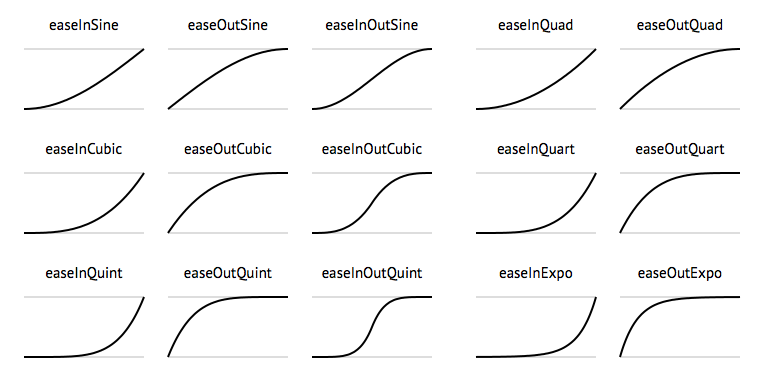
\includegraphics[width=1\textwidth]{easeing}
    \end{subfigure}

    \caption{Funções comumente usadas em interpolações de valores\label{fig:subfigures} (Imagem retirada do artigo de~\cite{VideoGameJuice})}
\end{figure}

O uso de \textit{tweens} se torna extremamente aparente quando utilizamos funções quadráticas, cúbicas, senoidais ou até mesmo elásticas para realizarmos a interpolação. Este efeito pode ser visto, por exemplo, no uso da bomba. Quando uma bomba é utilizada, uma circunferência (efeito da explosão) envolvendo a nave é rapidamente desenhada, tendo seu raio aumentado através de um \textit{tween} baseado em uma função cúbica. Após algumas frações de segundos, o raio da circunferência passa a ser aumentado em uma taxa consideravelmente menor, até finalmente parar e desaparecer, passando assim a imagem de uma explosão para o jogador.

Já não dependendo tanto dos \textit{tweens}, alguns dos \textit{sprites} de balas utilizados no jogos possuem um formato similar a de um losango achatado, com o intuito de clareza quanto à direção em que a bala se move. Balas circulares, por outro lado, podem deixar o entendimento de sua direção mais difícil para o jogador, e por conta disso são utilizadas mais frequentemente por chefes e sub-chefes.

Não se limitando aos visuais, a expressividade do jogo depende também de como os efeitos sonoros são utilizados. Eventos como \textit{ganhar uma vida} e \textit{ganhar uma bomba} são convenientemente demonstrados através de um efeito sonoro curto, distintos entre si, podendo também ser acompanhados de um pequeno indicador visual acima da nave. Neste caso, o \textit{tweening} também se mostra conveniente para suavizar a animação do texto (algo como \textit{Life up!} ou \textit{Bomb get!}) para cima e tornar o evento menos engessado.

% indicadores de qualquer coisa, mencionar a dificuldade depois só

% Variações em tempo real dos visuais gerais do jogo podem se mostrar úteis para indicação 